% !TEX root = master.tex
\chapter{Kickoff}
%Und los geht‘s – Startschuss zusammen mit den wichtigsten Kunden
%– Da das Projekt aufgrund von Kundenbeschwerden initiiert wurde und diese wiederum in
%einer Pilotphase mitwirken sollen, wurde ein gemeinsamer Kickoff beschlossen
%– Annahme: keine Pandemie
%– Aufgrund der weiten Anreise-Wege wurde beschlossen, den Kickoff in einem Workshop-
%Format stattfinden zu lassen:
%• Mind. 1 ganzer Tag, max. 2 ganze Tage Workshop
%• Durchführung am Hauptstandort der CP Service GmbH
%– Plant den Kickoff Workshop:
%• Wer sind die Stakeholder (+ Stakeholder-Analyse), welche Rollen sollen jeweils am
%Workshop teilnehmen?
%• Wie sieht die Agenda aus (und warum habt ihr euch dafür entschieden)?
%• Was ist zu organisieren, welches Material wird benötigt?
%• Wie sieht der Einladungstext an die Teilnehmer aus?
\label{chapter:5}
\section{Stakeholderanalyse}
Um die Durchführung des Kickoffs für das Projekt planen zu können, müssen relevante Stakeholder zu Beginn identifiziert und analysiert werden, sodass die Entwicklung passender Maßnahmen möglich ist. Stakeholder umfassen die Auftraggeber des Projektes, Beteiligte inklusive direkte betroffener Personen und sämtliche Akteure im Projektumfeld. In Tabelle \ref{tab:stakeholder} werden relevante Stakeholder für das Projekt der CP Service GmbH identifiziert und deren Erwartungen, Einstellung und Einfluss differenziert dargestellt. Dieser Ansatz ermöglicht eine initiale Kategorisierung der Stakeholder, um anschließende Maßnahmen ableiten zu können. Während \textit{\textquotedbl- -\textquotedbl} für eine behindernde Einstellung und geringe Einflussmöglichkeiten steht, bedeutet \textit{\textquotedbl-/+\textquotedbl} eine neutrale Einstellung mit mittleren Einflussmöglichkeiten. Es wird \textit{\textquotedbl++\textquotedbl} gewählt, wenn der Stakeholder das Projekt fördert oder hohe Einflussmöglichkeiten hat.
\vspace{10pt}


\begin{longtable}{|>{\arraybackslash}p{2.2cm}|>{\arraybackslash}p{5.7cm}|>{\centering\arraybackslash}p{0.5cm}|>{\centering\arraybackslash}p{0.7cm}|>{\centering\arraybackslash}p{0.5cm}|>{\centering\arraybackslash}p{0.5cm}|>{\centering\arraybackslash}p{0.7cm}|>{\centering\arraybackslash}p{0.5cm}|}
	\hline
	\textbf{Stakeholder} & \textbf{Erwartungen} & \multicolumn{3}{c|}{\textbf{Einstellung}} & \multicolumn{3}{c|}{\textbf{Einfluss}} \\ 
	\cline{3-8}
	& & - - & -/+ & ++ & - - & -/+ & ++ \\
	\hline
	\endfirsthead
	\multicolumn{8}{c}%
	{\tablename\ \thetable\ -- \textit{Fortsetzung von vorheriger Seite}} \\
	\hline
	\textbf{Stakeholder} & \textbf{Erwartungen} & \multicolumn{3}{c|}{\textbf{Einstellung}} & \multicolumn{3}{c|}{\textbf{Einfluss}} \\
	\cline{3-8}
	& & - - & -/+ & ++ & - - & -/+ & ++ \\
	\hline
	\endhead
	\hline \multicolumn{8}{r}{\textit{Weiter auf nächster Seite}} \\
	\endfoot
	\hline
	\endlastfoot
	
	Geschäfts-führer & Priorität hat die schnelle und qualitativ hochwertige Schnittstellenentwicklung. Die Lieferung muss fristgerecht sein und Budgets eingehalten werden. Das Ziel liegt in der Befriedigung der Großkunden.  & & & \checkmark & & & \checkmark\\ 
	\hline
	
	Poststelle & Klare Kommunikation über anstehende Veränderungen in ihrer Arbeit. Teilhabe an Weiterbildungsmöglichkeiten und Entwicklung von Übergangsprozessen. & \checkmark & & & \checkmark & & \\ 
	\hline
	
	Sach-bearbeiter & Erleichterungen und Effizienzsteigerungen durch das neue System. Ausreichende Schulungen sind notwendig, um mit der neuen Arbeitsweise vertraut zu werden und die Produktivität zu steigern. & & \checkmark & & & & \checkmark \\ 
	\hline
	
	Investoren \& Partner & Positiver ROI und Imagesteigerung als Kernelement. CP Service GmbH soll langfristig durch die Digitalisierung profitieren und Großkunden halten. Wollen über aktuelle Lagen informiert bleiben. & & \checkmark & & & \checkmark & \\ 
	\hline
	
	Großkunden & Beschleunigung der Prozesse durch Digitalisierung der Schnittstellen. Eigene Mitarbeiter sollen Anfragen direkt versenden können. Große Mitgestaltungsmöglichkeiten im Projekt werden erwartet, um Bedürfnisse durchzusetzen. & & & \checkmark & & & \checkmark \\ 
	\hline
	
	Projektteam & Eindeutig definierte Anforderungen des Projekts, um die Vision genau zu verstehen und umsetzen zu können. Eine vollständige Unterstützung durch die Geschäftsführung mit ausreichenden Ressourcen wird vorausgesetzt. & & \checkmark & & & & \checkmark \\ 
	\hline
	
	Compliance-Beauftragter & Einhaltung aller geltenden Datenschutzgesetze und -vorschriften für Kunden und Mitarbeiter. & & \checkmark & & & \checkmark & \\ 
	\hline
	
	Handels-ketten \& Kredit-institute & Erwarten eine höhere Effizienz in der Verarbeitung. Womöglich anschließende Digitalisierung anderer Bereiche. & & \checkmark & & \checkmark & & \\ 
	\hline
\end{longtable}
\captionof{table}{Stakeholder Analyse} \label{tab:stakeholder}
\vspace{20pt}

Die identifizierten Stakeholder unterscheiden sich mitunter deutlich in deren Erwartungen, Einstellung und Einfluss auf das Projekt. Während die Mehrheit der Stakeholder eine fördernde Einstellung vertritt, haben die Mitarbeiter der Poststelle die Befürchtung eines Arbeitsplatzverlusts, da deren Dienste bei einer Automatisierung nicht mehr notwendig sind. Um die einzelnen Stakeholder analysieren zu können und anschließend entsprechende Maßnahmen zu entwickeln, kategorisiert Abbildung \ref{fig:macht_cluster} diese bezüglich deren Konfliktpotential, Interesse und Macht. 
\vspace{10pt}

\begin{figure}[h]
	\centering
	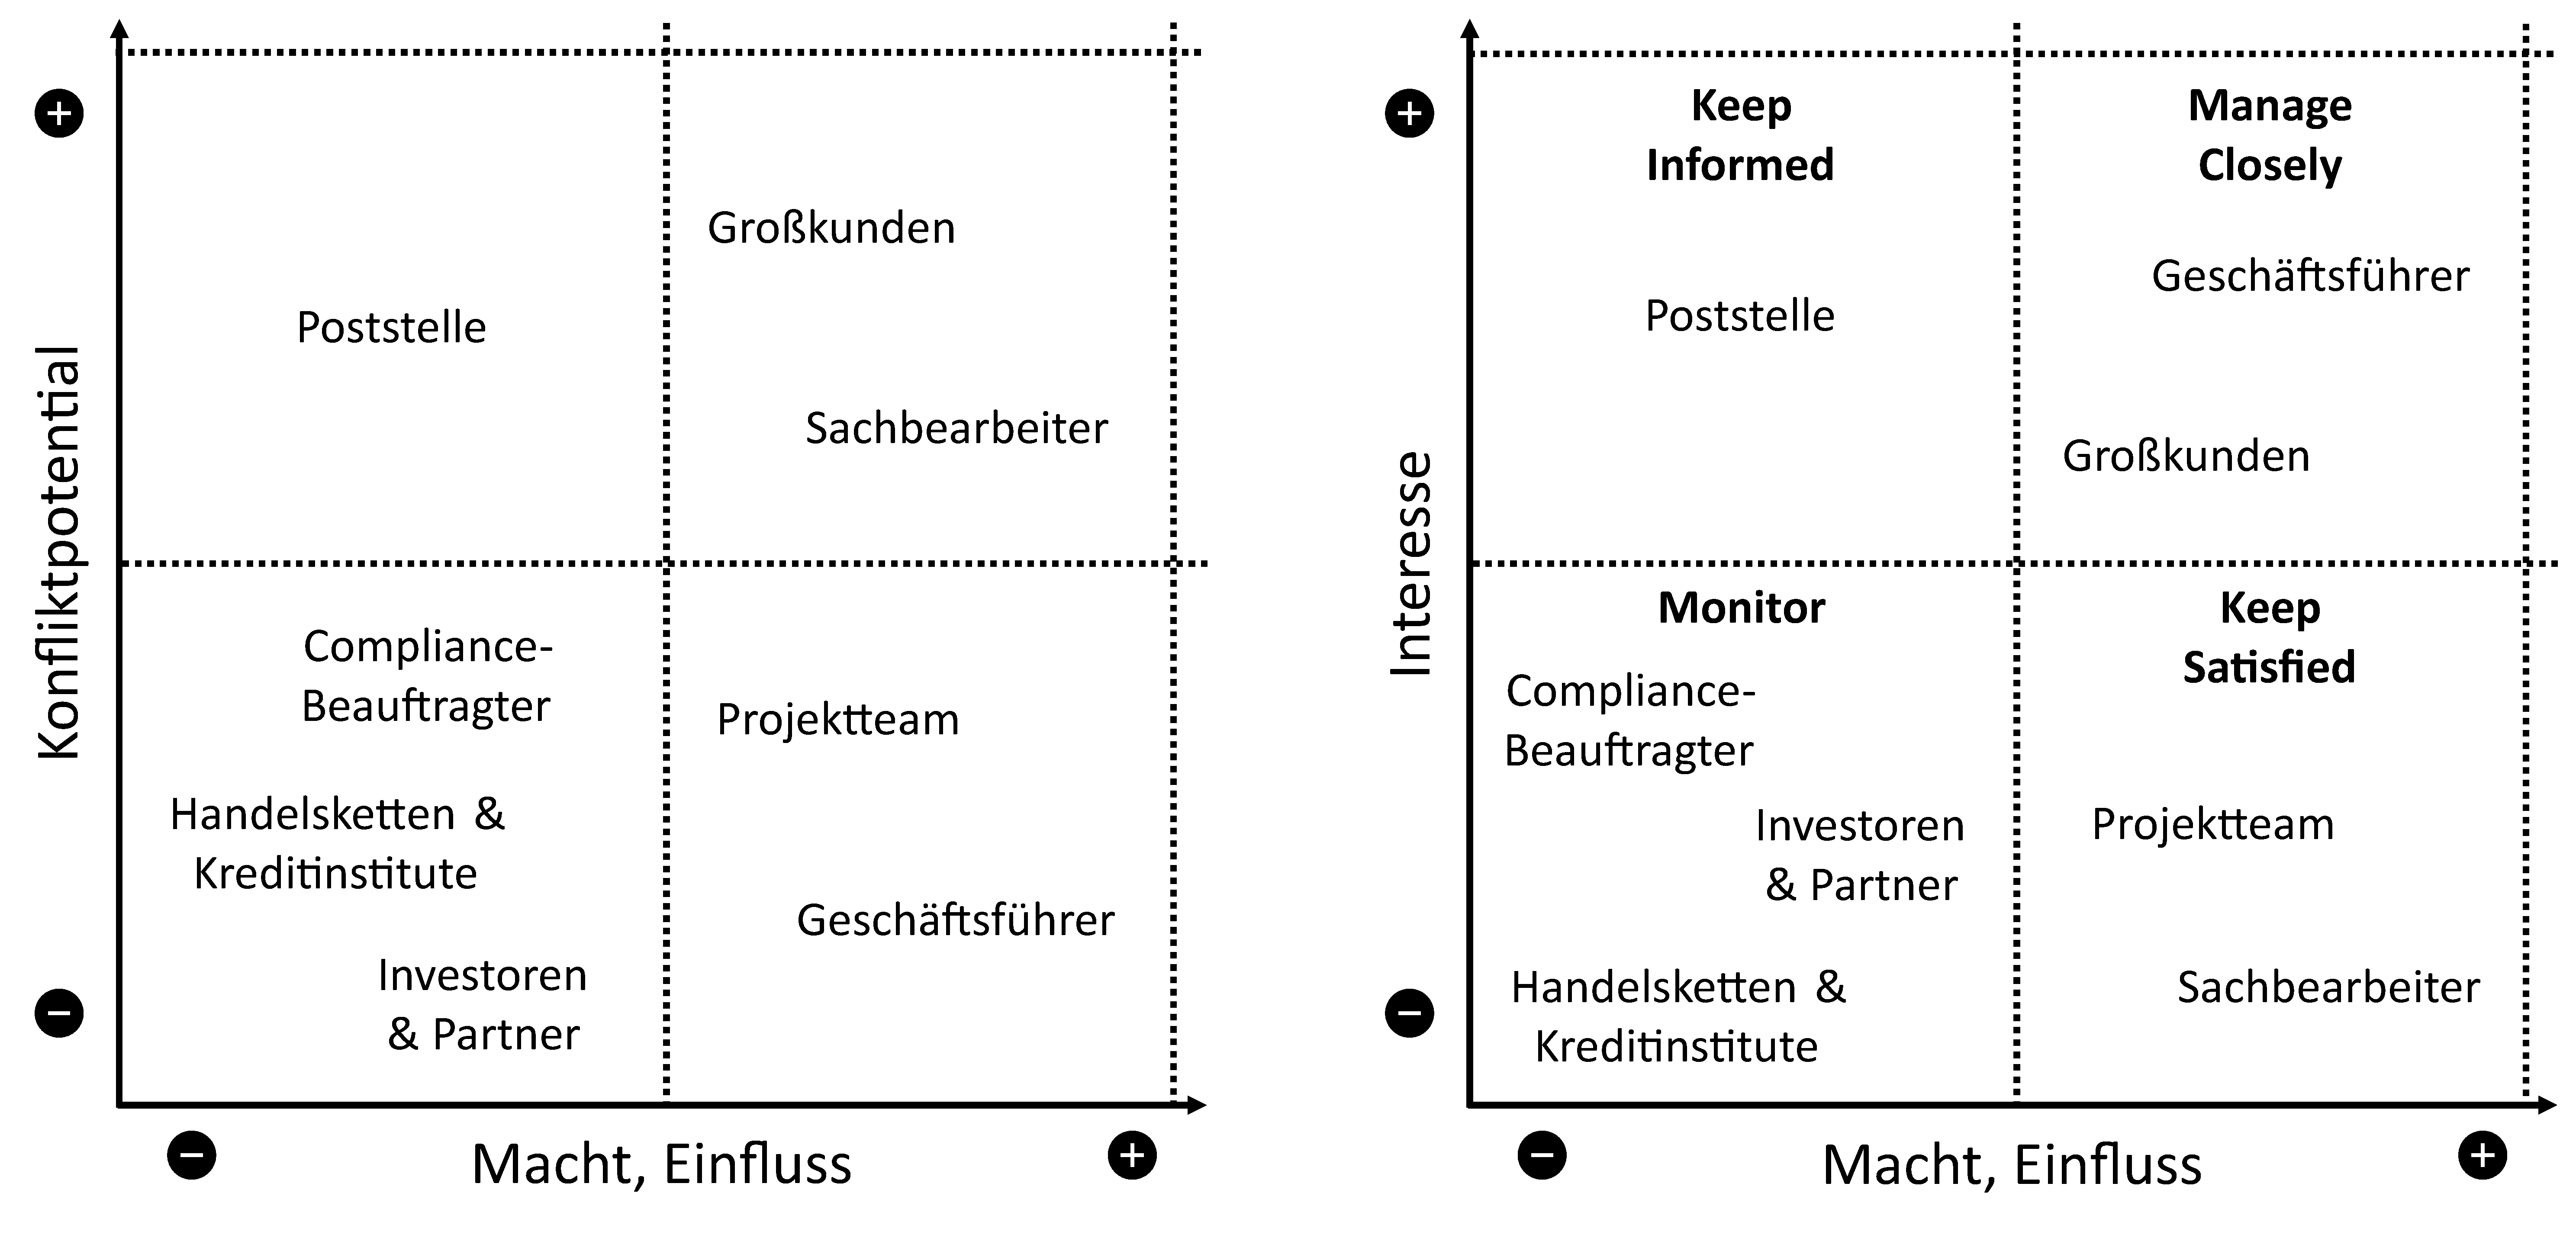
\includegraphics[width=\linewidth]{img/clustering.pdf}
	\caption{Kategorisierung der Stakeholder nach Konfliktpotential, Interesse und Macht}
	\label{fig:macht_cluster}
\end{figure}

Bei der Einteilung zwischen Konfliktpotential und Einflussmöglichkeiten der Stakeholder wird deutlich, dass die Großkunden und Sachbearbeiter über großen Einfluss und ein hohes Konfliktpotential verfügen. Die Großkunden haben die Umsetzung des Projektes vehement gefordert und möchten eigene Anforderungen umgesetzt haben. Durch die bereits erhaltenen Kündigungsdrohungen ist ein hohes Konfliktpotential gegeben. Die Sachbearbeiter hingegen werden nach Fertigstellung des Projekts mit dessen Produkt tagtäglich arbeiten. Somit haben diese einen großen Einfluss auf die Gestaltung, allerdings mit hohem Konfliktpotential, da vermutlich weitergehende, nicht umsetzbare Anforderungen gestellt werden. Die Geschäftsführung und das Projektteam haben ebenfalls einen hohen Einfluss auf das Projekt, allerdings ist das Konfliktpotential überschaubar. Beide Parteien sind direkt an der Projektplanung und dessen Umsetzung beteiligt und können eigene Ideen sofort einbringen. Die Mitarbeiter der internen Poststelle weisen hingegeben ein hohes Konfliktpotential mit relativ geringen Einflussmöglichkeiten auf. Diese sind direkt von den Veränderungen betroffen, da deren Arbeit wegfällt. Allerdings haben sie keine Möglichkeit, etwas hieran zu ändern. Die Investoren \& Partner, Handelsketten \& Kreditinstitute und Compliance-Beauftragte des Unternehmens haben wenig Einfluss und lediglich ein geringes Konfliktpotential, da sie höchstens indirekt durch das Projekt betroffen sind. Folgende Maßnahmen müssen sich daher insbesondere auf die zuvor genannten Stakeholder fokussieren, um deren Konfliktpotential zu minimieren.
\vspace{10pt}

Die Einordnung der Stakeholder bezüglich deren Interesse und Einflussmöglichkeiten ermöglicht eine Zuordnung der Quadranten \textit{Monitor} für wenig Interesse bei geringem Einfluss, \textit{Keep Informed} für viel Interesse bei geringer Macht, \textit{Keep Satisfied} für wenig Interesse bei hoher Macht und \textit{Manage Closely} für viel Interesse bei hoher Macht. Es ergeben sich ähnliche Zusammenhänge im Vergleich zur Kategorisierung nach dem Konfliktpotential, wobei primär die Quadranten \textit{Manage Closely} und \textit{Keep Satisfied} von Relevanz sind. Die Geschäftsführung und Großkunden haben beide direkte Interessen und einen starken Einfluss auf das Projekt. Da die Projektdurchführung von den Großkunden mit Vehemenz gefordert wurde, ist es für die Geschäftsführung von zentraler Bedeutung dieses mit Erfolg umzusetzen. Hingegen befinden sich Projektteam und Sachbearbeiter lediglich im Quadranten \textit{Keep Satisfied}. Für das Projektteam ist dies mit der geringen Dauer des Projekts und der Teamzusammensetzung aus externen und internen Mitarbeitern zu begründen. Die Sacharbeiter haben zudem auch nur ein limitiertes Interesse, da die Umsetzung des Projektes gleichbedeutend mit dem Zwang zur Veränderung und Anpassung ist. Routinen und gelernte Prozesse müssen überarbeitet und neu gelernt werden, weshalb eine gewisse Anfangshürde besteht.
\vspace{10pt}

Basierend auf den identifizierten und analysierten Stakeholdern müssen unterschiedliche Maßnahmen ergriffen werden, um mit diesen in differenzierten Weisen umzugehen. Diese unterscheiden sich in Sofortmaßnahmen und Vorsorgepläne \& Strategien. Hierbei stellen Sofortmaßnahmen Reaktionen auf aktuelle oder unmittelbar bevorstehende Ereignisse oder Probleme dar und müssen daher schnell umgesetzt werden. Sie zielen darauf ab, unmittelbare Risiken zu mindern, Konflikte zu vermeiden und eine positive Beziehung zu den Stakeholdern aufrechtzuerhalten. Vorsorgepläne \& Strategien hingegen beziehen sich auf langfristige Maßnahmen und Pläne, um potenzielle zukünftige Herausforderungen oder Möglichkeiten anzugehen. Die Beziehung zu den Stakeholdern soll über die gesamte Projektlaufzeit positiv und effektiv gestaltet sein. Tabelle \ref{tab:maßnahmen} stellt die Sofortmaßnahmen und Vorsorgepläne \& Strategien als Maßnahmenkatalog dar.
\vspace{10pt}

\begin{longtable}{|p{2.2cm}|p{5.7cm}|p{5.6cm}|}
	\hline 
	\textbf{Stakeholder} & \textbf{Sofortmaßnahmen} & \textbf{Vorsorgepläne \& Strategien} \\
	\hline 
	\endfirsthead
	\multicolumn{3}{c}%
	{\tablename\ \thetable\ -- \textit{Fortsetzung von vorheriger Seite}} \\
	\hline 
	\textbf{Stakeholder} & \textbf{Sofortmaßnahmen} & \textbf{Vorsorgepläne und Strategien} \\
	\hline 
	\endhead
	\hline \multicolumn{3}{r}{\textit{Weiter auf nächster Seite}} \\
	\endfoot
	\hline
	\endlastfoot
	Geschäfts-führung & Einführung in das Projekt und Erläuterung der Ziele und des Zeitplans. & Regelmäßige Updates und Meetings zur Diskussion von Fortschritten und Hindernissen \\
	\hline
	Sach-bearbeiter & Workshops zur Ausarbeitung aller relevanten Anforderungen und Erläuterungen der zu erwartenden Veränderungen & Enge Integration in der Anforderungsaufnahme und im Testen der Anwendung. Schulungen und weitere Unterstützung während des Übergangsprozesses \\
	\hline
	Poststelle & Information über die bevorstehenden Änderungen und Diskussion über die Auswirkungen auf ihre Arbeit & Entwicklung eines Übergangsplans, um die Änderungen zu erleichtern \\
	\hline
	Großkunden & Information über das neue System und dessen Vorteile, Diskussionen und Workshops über deren Bedürfnisse und Erwartungen & Fortlaufende Kommunikation und Unterstützung während des Übergangs, Anpassung des Systems basierend auf deren Feedback \\
	\hline
	Compliance-Beauftragter & Frühzeitige Einbindung in den Planungsprozess, um die Erfüllung aller Datenschutzanforderungen sicherzustellen & Kontinuierliche Überprüfung der Datenschutzmaßnahmen während der Projektumsetzung \\
	\hline
	Projektteam & Bereitstellung von ausreichenden Ressourcen und klare Kommunikation der Projektziele, -erwartungen und -anforderungen & Fortlaufende Unterstützung und Ressourcenmanagement während des gesamten Projekts \\
	\hline
	Externe Partner \& Investoren & Offizielle Mitteilung über das neue Projekt und dessen Ziele & Regelmäßige Updates über den Fortschritt des Projekts \\
	\hline
	Handels-ketten \& Kredit-institute & Offizielle Mitteilung über das neue Projekt und dessen Vorteile & Regelmäßige Updates über den Fortschritt des Projekts \\
	\hline
\end{longtable}
\captionof{table}{Maßnahmenkatalog für Umgang mit Stakeholdern} \label{tab:maßnahmen}
\vspace{20pt}

Für die Kommunikation mit den unterschiedlichen Stakeholdern bedarf es einer Differenzierung in den gewählten Kommunikationsstrategien. Hierbei wird zwischen partizipativem, diskursivem und repressivem Vorgehen unterschieden. Das partizipative Vorgehen bindet den Stakeholder aktiv in Entscheidungsprozesse ein, wodurch das Gefühl der Einflussnahme entsteht. Dies ist von besonderer Relevanz, wenn der Stakeholder direkt von den Entscheidungen betroffen ist oder dessen spezifisches Wissen benötigt wird. Sowohl für die internen Sachbearbeiter, als auch für die Großkunden wird daher das partizipative Vorgehen gewählt, da die Umsetzung derer Anforderungen und die Befriedigung derer Bedürfnisse unerlässlich ist. Für das Projektteam wird ebenfalls dieses Vorgehen gewählt, da es unmittelbar an der Entwicklung und Umsetzung des Projekts beteiligt ist und eine aktive Beteiligung somit gegeben ist. Bei dem diskursivem Vorgehen steht der Austausch und die Diskussionen von Ideen im Vordergrund. Es wird gewählt, wenn die Stakeholder eine hohe Autorität oder Einfluss auf das Projekt haben und unterschiedliche Meinungen hin zu einem Konsens berücksichtigt werden müssen. Diese Kommunikationsstrategie wird daher für die Geschäftsführung genutzt, da diese strategische Entscheidungen trifft, welche umzusetzen sind. Auch für die interne Poststelle und die Datenschutzbeauftragten wird diese Strategie gewählt, um deren Bedenken, Vorschläge und Tipps einbringen zu können. Für die Partner \& Investoren und die Handelsketten \& Kreditinstitute ist diese Strategie ebenfalls von Vorteil, da diese ein Interesse am Projekt haben und sich deren Unterstützung als hilfreich entpuppen kann. Das repressive Vorgehen hingegen nutzt eine intransparente und einseitige Kommunikationsstruktur, um die Offenlegung der Informationen zu verhindern. Da es sich bei unserem Projekt weder um geheime Forschung, noch um anderweitig vertrauliche Themen handelt, wird diese Strategie für keinen Stakeholder verwendet.


\section{Agenda des Kickoff-Workshops}

Basierend auf der durchgeführten Stakeholderanalyse beginnt nun die Planung des Kickoff-Workshops. Alle Schlüsselstakeholder werden zu dem Kickoff-Workshop eingeladen, um Projektziele und Erwartungen zu verdeutlichen und die Zusammenarbeit zu fördern. Dies umfasst die Geschäftsführung, Sachbearbeiter, Großkunden, Datenschutzbeauftragte und das Projektteam. Die Aufgabe der Geschäftsführung während des Kickoff-Workshops liegt in der Erklärung der strategischen Auslegung und Relevanz des Projektes, um alle Teilnehmenden zu motivieren und Unterstützung zu signalisieren. Die Sacharbeiter und Großkunden sind als Endnutzer ebenfalls von Bedeutung, da diese letztendlich mit der entwickelten Lösung arbeiten werden. Bedürfnisse, Anforderungen und Feedback dieser Stakeholder ist daher während des Workshops zu erheben und in der Planung einzuarbeiten. Die Teilnahme des Projektteams ist ebenfalls unverzichtbar, da diese das Projekt umsetzen werden. Während des Workshops können daher Unklarheiten geklärt und Begeisterung für das Projekt geschaffen werden. Auch ein Datenschutzbeauftragter des Unternehmens wird als Unterstützung im Kickoff teilnehmen. Dieser kann sicherstellen, dass alle Datenschutzanforderungen von Beginn an berücksichtigt werden und als Experte für Fragen in diesem Bereich fungieren. Es wird sich bewusst gegen die Einladung von Mitarbeitern der internen Poststelle entschieden, da Arbeitserfahrungen dieser nicht relevant für das Projekt sind. Zudem wären Beitrage der Poststelle eher negativer Natur, da diese um den Verlust ihrer Arbeitsplätze fürchten. Dies würde einen kontraproduktiven Beitrag zum Kickoff-Workshop darstellen, sodass die Produktivität und Effizienz aller Teilnehmenden hierunter leiden würde. Auch externe Partner \& Investoren und Handelsketten \& Kreditinstitute werden aufgrund ihrer Distanz zum Projekt nicht eingeladen. Insgesamt wird mit der Teilnahme von 15 Personen gerechnet, welche sich aus einem Vertreter der Geschäftsführung, dem Projektleiter, drei Vertretern der Großkunden, drei Sachbearbeitern, einem Datenschutzbeauftragten und dem Projektteam der Größe von 6 Mitarbeitern zusammensetzt.
\vspace{10pt}

Bevor die Einladung des Kickoff-Workshop versendet werden kann, muss eine Agenda ausgearbeitet sein. Aufgrund der weiten Anreise mancher Stakeholder wird der Workshop für zwei Tage geplant. Dies ist sinnvoll, da der Kickoff-Workshop wegweisend für das gesamte Projekt ist und eine produktive Zusammenarbeit aller Beteiligten dadurch ermöglicht wird. Der Workshop findet im internen Schulungszentrum der CP Service GmbH statt, welches zahlreiche Ressourcen im Vorhinein bereitstellt. Tabelle \ref{tab:agenda} zeigt die Agenda für den Workshop. Der gesamte Kickoff-Workshop wird durch den Projektleiter Franz Bauer geleitet, um dessen Führungsqualitäten allen Teilnehmern demonstrieren zu können.

\clearpage
\begin{center}
	\Large{\textbf{Tag 1}}
\end{center}

\noindent
\begin{tabularx}{\textwidth}{@{}lX@{}}
	08:30-09:00 & \textbf{Eintreffen der Teilnehmer}\\
	09:00-09:30 & \textbf{Begrüßung und Vorstellung}\\
	& Überblick über den Workshop und die Vorstellung der Teilnehmer.\\
	09:30-10:15 & \textbf{Projektüberblick}\\
	& Präsentation des Projekts, dessen Ziele und des erwarteten Nutzens.\\
	10:15-10:30 & \textbf{Kaffeepause}\\
	10:30-12:00 & \textbf{Diskussion: Projektziele und Erwartungen der Stakeholder}\\
	& Erwartungen und Bedürfnisse der verschiedenen Stakeholder.\\
	12:00-13:00 & \textbf{Mittagspause}\\
	13:00-14:30 & \textbf{Präsentation: Projektplan und -strategie}\\
	& Präsentation des Projektzeitplans und der geplanten Maßnahmen.\\
	14:30-15:00 & \textbf{Kaffeepause}\\
	15:00-16:00 & \textbf{Workshop: Beteiligung der Stakeholder}\\
	& Ausarbeitung von Möglichkeiten der Zusammenarbeit.\\
	16:00-16:30 & \textbf{Closing}\\
	16:30- o.e. & \textbf{[Optional] Gemeinsames Abendessen}
\end{tabularx}


\begin{center}
	\Large{\textbf{Tag 2}}
\end{center}

\noindent
\begin{tabularx}{\textwidth}{@{}lX@{}}
	09:00-09:15 & \textbf{Begrüßung und Überblick}\\
	09:15-10:30 & \textbf{Workshop: Identifizierung möglicher Hindernisse und Risiken}\\
	& Ausarbeitung von Risiken und Entwicklung von Lösungsstrategien.\\
	10:30-10:45 & \textbf{Kaffeepause}\\
	10:45-12:00 & \textbf{Diskussion: Umgang mit Änderungen und Unsicherheiten}\\
	& Änderungsmanagement und der Umgang mit Unsicherheiten.\\
	12:00-13:00 & \textbf{Mittagspause}\\
	13:00-14:30 & \textbf{Diskussion: Verantwortlichkeiten und Rollen im Projekt}\\
	& Rollen und Verantwortlichkeiten der verschiedenen Stakeholder.\\
	14:30-14:45 & \textbf{Kaffeepause}\\
	14:45-16:00 & \textbf{Abschlussdiskussion und nächste Schritte}\\
	& Diskussion der nächsten Schritte und Abschluss des Workshops.\\
\end{tabularx}

\captionof{table}{Agenda für den zweitägigen Kickoff-Workshop}
\label{tab:agenda}
\clearpage

Obwohl der offizielle Beginn des Kickoff-Workshops um 9:00 Uhr ist, muss bereits für die Zeit davor geplant werden. Die Teilnehmer haben eine lange Anreise und werden teilweise bereits vor dem offiziellen Beginn ankommen und einander kennenlernen. Hierfür ist eine entspannte und gemütliche Atmosphäre von Vorteil, sodass die Teilnehmer mit einem positiven Gefühl in den Workshop starten. Es ist wichtig, dass insbesondere für die externen Teilnehmer eine klare Wegbeschreibung zum Schulungszentrum der CP Service GmbH gegeben ist. Diese sollten anschließend von Personal empfangen und zum Raum begleitet werden. Der Projektleiter, welcher den Workshop leiten wird, muss bereits anwesend und der Raum vorbereitet sein. Um eine entspannte Atmosphäre zu schaffen, müssen Snacks, frische Früchte und Getränke jederzeit bereitstehen, um alle Anwesenden zu verpflegen. Der Schulungsraum muss einen großen Tisch in der Mitte haben, an welchen sich alle Teilnehmenden setzen werden. Während beider Tage sind zahlreiche Pausen eingeplant. Diese dienen zum einen der Erholung und Verarbeitung erarbeiteter Themen, sind aber umso wichtiger für das Vernetzen der einzelnen Teilnehmer. Das gesamte Projekt profitiert von einer möglichst guten Zusammenarbeit zwischen den einzelnen Stakeholdern und diese wird durch ein gemeinsames Kennenlernen stark gefördert. 
\vspace{10pt}

Sobald alle Teilnehmer um 9:00 Uhr eingetroffen sind, begrüßt der Projektleiter diese und initiiert eine Vorstellungsrunde. Hierbei ist es wichtig, dass neben beruflichen Aspekten ebenfalls etwas auf private Interessen eingegangen wird, um gemeinsame Gesprächsthemen zu finden und soziale Verbindungen zu knüpfen. Dies soll der emotionalen Auflockerung des Workshops dienen und die Atmosphäre positiv beeinflussen. Nach der Vorstellungsrunde beginnt um 9"30 Uhr der Projektleiter gemeinsam mit der Geschäftsführung einen Überblick über das Projekt, dessen Ziele und den erwarteten Nutzen zu geben. Die Geschäftsführung muss hierbei eine aktive Rolle in der Präsentation einnehmen, um die starke Unterstützung der Führungsspitze zu verdeutlichen. Das Ziel liegt sowohl in der Übermittlung zentraler Projektinformationen, als auch in der Schaffung von Motivation und Begeisterung aller Beteiligter. Nach einer anschließenden Kaffeepause wird um 10:30 Uhr eine aktive Diskussion über Projektziele und Erwartungen der Stakeholder initiiert. Hierbei sollen alle Bedürfnisse offengelegt und klar kommuniziert werden. Dieser Schritt ist von hoher Relevanz, da das Projektteam die konkreten Anforderungen der Großkunden und Sachbearbeiter aufnehmen und verstehen können, sodass eine anschließende Annahme der Anwendersicht möglich wird. Da vermutlich nicht alle Erwartungen umsetzbar sind, muss der Projektleiter als Moderator fungieren und die Diskussion geschickt lenken. Zudem muss sichergestellt werden, dass alle Teilnehmenden aktiv mitarbeiten und nicht einzelne Teilnehmer sämtliche Redeanteile besitzen. Nach der Mittagspause folgt dann um 13:00 Uhr die Präsentation des Projektplans und der Projektstrategie. Der Projektzeitplan wird vorgestellt und geplante Maßnahmen durch den Projektleiter erläutert, sodass alle Teilnehmenden tiefe Einblicke in die Planung erhalten und sich eingebunden fühlen. Da diese Präsentation zahlreiche Informationen vermittelt, wird anschließend eine große Kaffeepause gemacht, in welcher sich die Teilnehmenden auf der Dachterrasse entspannen können. Danach wird noch um 15:00 Uhr ein interaktiver Workshop über die Beteiligung der Stakeholder durchgeführt. Hierbei wird der Projektleiter eine Diskussion über die Rollenverteilung der verschiedenen Stakeholder im Projekt moderieren und gemeinsam mit den Teilnehmenden die Möglichkeiten zur Zusammenarbeit ausarbeiten. Nach diesem Workshop findet um 16:00 Uhr noch das Closing durch den Projektleiter ab, welches die Ergebnisse des ersten Tags zusammenfasst und auf zukünftige Themen eingeht. Dieses Closing beendet den offiziellen Teil des ersten Tages, allerdings wird es für alle Teilnehmenden möglich sein, sich auf ein entspanntes gemeinsames Abendessen in der Stadt zu treffen, um den Tag ausklingen zu lassen.
Nach dem Ende des ersten Tages bereitet der Projektleiter die erzielten Ergebnisse nach und analysiert diese, um langfristig hiervon zu profitieren.
\vspace{10pt}

Der zweite Tag des Kickoff-Workshops beginnt erneut um 9:00 Uhr mit einer Begrüßung durch den Projektleiter. Hierbei wird erneut ein Überblick über bevorstehende Aktivitäten des Tages gegeben, sodass alle Teilnehmenden die Struktur und Organisation des Tages verdeutlicht bekommen. Anschließend beginnt um 9:15 Uhr die Ausarbeitung der Identifikation möglicher Hindernisse und Risiken, um sich dessen bewusst zu werden. Dies ist erneut als aktiver Workshop aufgebaut, in welchem die Teilnehmer ins gemeinsame Gespräch kommen. Risiken und Lösungsstrategien werden gemeinsam ausgearbeitet und anschließend dokumentiert. Der Projektleiter nimmt hierbei eine passivere Rolle an, um den Teilnehmenden mehr Spielraum zu ermöglichen, sodass diese auf neue Ideen kommen können. Nach einer kurzen Kaffeepause wird eine zweite Diskussion um 10:45 Uhr durchgeführt, in welcher es um den Umgang mit Änderungen und Unsicherheiten geht. Die Großkunden und Sachbearbeiter werden starke Veränderungen in ihrem Arbeitsalltag erleben, weshalb diese im Fokus stehen. Es ist auszuarbeiten, inwiefern diese unterstützt und geschult werden können, um die neue Produktlösung nahtlos integrieren zu können. Nach der Mittagspause kommt es um 13:00 Uhr zu einer weiteren Präsentation mit einhergehender Diskussion über die Verantwortlichkeiten und Rollen im Projekt. Hierbei müssen die Befugnisse und Verantwortlichkeiten der einzelnen Stakeholder und deren Einfluss geklärt werden. Es ist erneut wichtig, dass die Geschäftsführung ein positives Bild vermittelt und die vollständige Unterstützung des Projektes signalisiert. Nach einer weiteren Kaffeepause beginnt anschließend die Abschlussdiskussion, in welcher folgende Schritte abgeklärt werden. Nach Abschluss der Diskussion wird anschließend noch Sekt serviert, um den Projektstart zu feiern. Da es sich um den Tag der Abreise handelt und gegebenenfalls manche Teilnehmer noch mit dem Auto fahren, muss ebenfalls eine alkoholfreie Alternative angeboten werden. Der Tag endet somit mit einem positiven Gefühl und alle Teilnehmer können sich auf das Projekt freuen.

\section{Benötigte Materialien}
Der Kickoff-Workshop beinhaltet unterschiedliche Elemente wie Präsentationen, Diskussionen und gemeinsame Ausarbeitungen. Daher ergeben sich diverse benötigte Materialien, welche für den Kickoff-Workshop bereitgestellt werden müssen. Es ist zu beachten, dass die Kaffeemaschine bereits fest installiert ist und das Mittagessen in der Kundenkantine stattfindet, weshalb dies nicht mehr beachtet werden muss. Wie bereits im vorangegangenen Teil beschrieben, wird die Teilnahme von 15 Personen erwartet. Tabelle \ref{tab:materialien} listet alle benötigten Materialien auf, welche für die Organisation des Kickoff-Workshops besorgt werden müssen.
\vspace{10pt}

\begin{table}[h]
	\centering
	\begin{tabular}{|l|l|}
		\hline
		\textbf{Materialien}             & \textbf{Anzahl/Beschreibung} \\
		\hline
		Beamer & 1 \\
		\hline
		Leinwand & 1 \\
		\hline
		Flipchart-Ständer & 3 \\
		\hline
		Flipchart-Papier & Mehrere Blätter \\
		\hline
		Marker (verschiedene Farben) & Mehrere Sätze \\
		\hline
		Post-It Notizen (verschiedene Farben) & Mehrere Päckchen \\
		\hline
		Whiteboard & 1 \\
		\hline
		Whiteboard-Marker & Mehrere Sätze \\
		\hline
		Notizblöcke & 1 pro Teilnehmer \\
		\hline
		Kugelschreiber & 2 pro Teilnehmer \\
		\hline
		Namensschilder & 1 pro Teilnehmer \\
		\hline
		Schilder für die Wegweisung im Gebäude & Mehrere \\
		\hline
		Tische & Ausreichend für alle Teilnehmer \\
		\hline
		Stühle & Ausreichend für alle Teilnehmer \\
		\hline
		Getränke (Wasser, Kaffee, Tee, Säfte) & Ausreichend für alle Teilnehmer \\
		\hline
		Snacks und frische Früchte & Ausreichend für alle Teilnehmer \\
		\hline
		(Alkoholfreier) Sekt für Abschlussfeier & Ausreichend für alle Teilnehmer \\
		\hline
	\end{tabular}
	\caption{Benötigte Materialien für den Kickoff-Workshop}
	\label{tab:materialien}
\end{table}

Neben den benötigten Materialien ist es zusätzlich wichtig, dass weitere Mitarbeiter für die Organisation eingespannt werden. Das Personal des Empfangs muss externe Teilnehmer zum Raum begleiten und es ist zusätzlich ein Praktikant oder Werkstudent notwendig, um bei der kontinuierlichen Dokumentation des Kickoff-Workshops zu unterstützen und ein Protokoll zu führen. Da es sich um einen zweitägigen Workshop handelt und die Vertreter der Großkunden einen weiten Anreiseweg haben, müssen für diese Unterkünfte organisiert werden. Die CP Service GmbH verfügt über ein kleines Kundenhotel in der Nähe des Schulungszentrums. Hier müssen Reservierungen für diese getätigt werden. 


\section{Einladungstext}
Nach der erfolgreichen Stakeholderanalyse, der entwickelten Agenda und ausgearbeiteten Materialien können nun Einladungen an die Stakeholder versendet werden. Da interne Mitarbeiter bereits vor dem Kickoff-Workshop einige Informationen über das Projekt erhalten, dient dieser Einladungstext primär externen Stakeholdern. Es wird versucht einen freundlich bestimmten Schreibstil zu nutzen und die Kompetenzen der einzelnen Stakeholder zu betonen. Es ist wichtig, dass dieser Einladungstext einen positiven Eindruck hinterlässt, sodass der Kickoff-Workshop erfolgreich sein kann. 

\begin{figure}[ht]
	\centering
	\begin{minipage}{\textwidth}		
		\noindent Sehr geehrter [Stakeholder],
		
		\vspace*{1.5\baselineskip}
		
		\noindent wie sie womöglich mitbekommen haben, wollen wir die CP Service GmbH das Projekt Digipaper starten, um Schnittstellen zu digitalisieren. Da wir von Ihrer Kompetenz überzeugt und Ihren Ideen begeistert sind, würden wir Sie sehr gerne zu unserem bevorstehenden \textbf{Kickoff-Workshop} einladen. Dieser findet am \textbf{15. und 16. November 2023} an unserem Hauptstandort in Mannheim statt. 
		
		\vspace*{0.5\baselineskip}
		
		\noindent Dieser Workshop bietet eine wertvolle Gelegenheit, uns gemeinsam auf das spannende Projekt vorzubereiten und unsere \textbf{Ziele und Erwartungen} für die bevorstehenden Monate zu klären. Die Agenda für den Workshop finden Sie im Anhang. 
		
		\vspace*{0.5\baselineskip}
		
		\noindent Während des Workshops wird ein großer Wert auf aktive Beteiligung aller Teilnehmer und deren Meinungen gelegt. Gemeinsam möchten wir die Eckpfeiler des Projekts definieren, unsere Strategie festlegen und mögliche Herausforderungen diskutieren. Sie sind herzlich eingeladen, \textbf{Ihre Ideen und Perspektiven} einzubringen.
		
		\vspace*{0.5\baselineskip}
		
		\noindent Während des Workshops stellen wir Getränke und Snacks sowie ein Mittagessen bereit, um sicherzustellen, dass Sie sich während des ganzen Tages wohlfühlen und konzentrieren können. Sofern eine Unterkunft benötigt wird, sind Sie herzlich dazu eingeladen in unserem Kundenhotel zu übernachten.
		
		\vspace*{0.5\baselineskip}
		
		\noindent Bitte lassen Sie uns bis zum \textbf{10. August 2023} wissen, ob Sie teilnehmen können. Falls Sie von außerhalb anreisen, senden wir Ihnen gerne eine Wegbeschreibung zum Schulungszentrum zu.
		
		\vspace*{0.5\baselineskip}
		
		\noindent Wir freuen uns sehr darauf, Sie bei diesem wichtigen Kickoff-Workshop begrüßen zu dürfen und sind zuversichtlich, dass wir gemeinsam ein erfolgreiches und produktives Projekt starten werden.
		
		\vspace*{1.5\baselineskip}
		
		\noindent Mit freundlichen Grüßen
		
		\vspace*{0.5\baselineskip}
		
		\noindent Franz Urlaub
		
		\noindent Projektleiter
		
		\vspace*{2\baselineskip}
		
		\caption{Einladungsschreiben für den Kickoff-Workshop}
		\label{fig:einladung} 
	\end{minipage}
\end{figure}









